\glsresetall
\chapter{State of the Art}
\label{chap:state_of_the_art}

In this Chapter, we discuss the core concepts regarding the project, the most modern technology for the purpose today and related work in the area. All the information presented results from work of research through published articles, knowledge exchange and web searching.

First, the main purpose of Section~\ref{sec:concepts}~-~\nameref{sec:concepts} is to introduce and provide a brief explanation about the core concepts to the reader. Second, Section~\ref{sec:technologies}~-~\nameref{sec:technologies}, all the relevant technologies are analysed and discussed. In the final Section~\ref{sec:related_work}~-~\nameref{sec:related_work}, published articles and posts of related work are presented and possible research directions are discussed.

\section{Concepts}
\label{sec:concepts}

The following concepts represents the baseline to understand the work related to this research project. First an explanation of higher level of concepts that composes the title of this thesis are presented in Subsections~\ref{subsec:microservices} and~\ref{subsec:observability_and_controlling_performance}. The following Subsections~\ref{subsec:distributed_tracing} to~\ref{subsec:time_series}, aim to cover topics  related to previous concepts:~\nameref{subsec:distributed_tracing}, ~\nameref{subsec:graphs} and~~\nameref{subsec:time_series}.

\subsection{Microservices}
\label{subsec:microservices}

The term ``micro web services'' was first used by Dr. Peter Rogers during a conference on cloud computing in 2005, and evolved later on to ``Microservices'' at an event for software architects in 2011, where the term was used to describe a style of architecture that many attendees were experimenting with at the time. Netflix and Amazon were among the early pioneers of microservices~\cite{MauersbergerMicroservices}.

Microservices is ``an architectural style that structures an application as a collection of loosely coupled services, which implement business capabilities''~\cite{Dragoni2017, microservices_definition}.

This style of software development has a very long history and has being introduced and evolving due to software engineering achievements in the later years regarding cloud distributed computing infrastructures, \gls{api} improvements, agile development methodologies and the emergence of the recent phenomenon of containerized applications. ``A container is a standard unit of software that packages up code and all its dependencies so the application runs quickly and reliably from one computing environment to another, communicating with others through an \gls{api}''~\cite{Pahl2017}.

In Microservices, services are small, specifically calibrated to perform a single function, also each service is designed to be autonomous, resilient, minimal and composable. This framework brings a culture of rapid iteration, automation, testing, and continuous deployment, enabling teams to create products and deploy code exponentially faster than ever before~\cite{Newman}.

%The core concept of microservices stands in isolation, or by other words, what everyone wants to achieve when building a software with microservices in mind, is to share less things between the services and deal with correlated failures. In this sense, a service is a small part of the entire system (e.g. Get messages microservice), and represents a tiny feature of the whole service (e.g. Chat Service). To do this, normally every microservice is encapsulated inside a container (e.g. Docker container~\cite{docker}), and each runs in its own process and communicates with the other using lightweight mechanisms, often an \gls{http} resource \gls{api}. 

Until the rising of Microservices based architecture, the Monolithic architectural style was the most used. This style has a the particularity of produce software composed all in one piece. All features are bundled, packaged and deployed in a single tier application using a single code base.

Figure~\ref{fig:monolithic_and_microservices} aims to give a comparison between both architectural styles, Monolithic and Microservices, and provide an insight about the differences between them.

\begin{figure}[H]
    \centering
    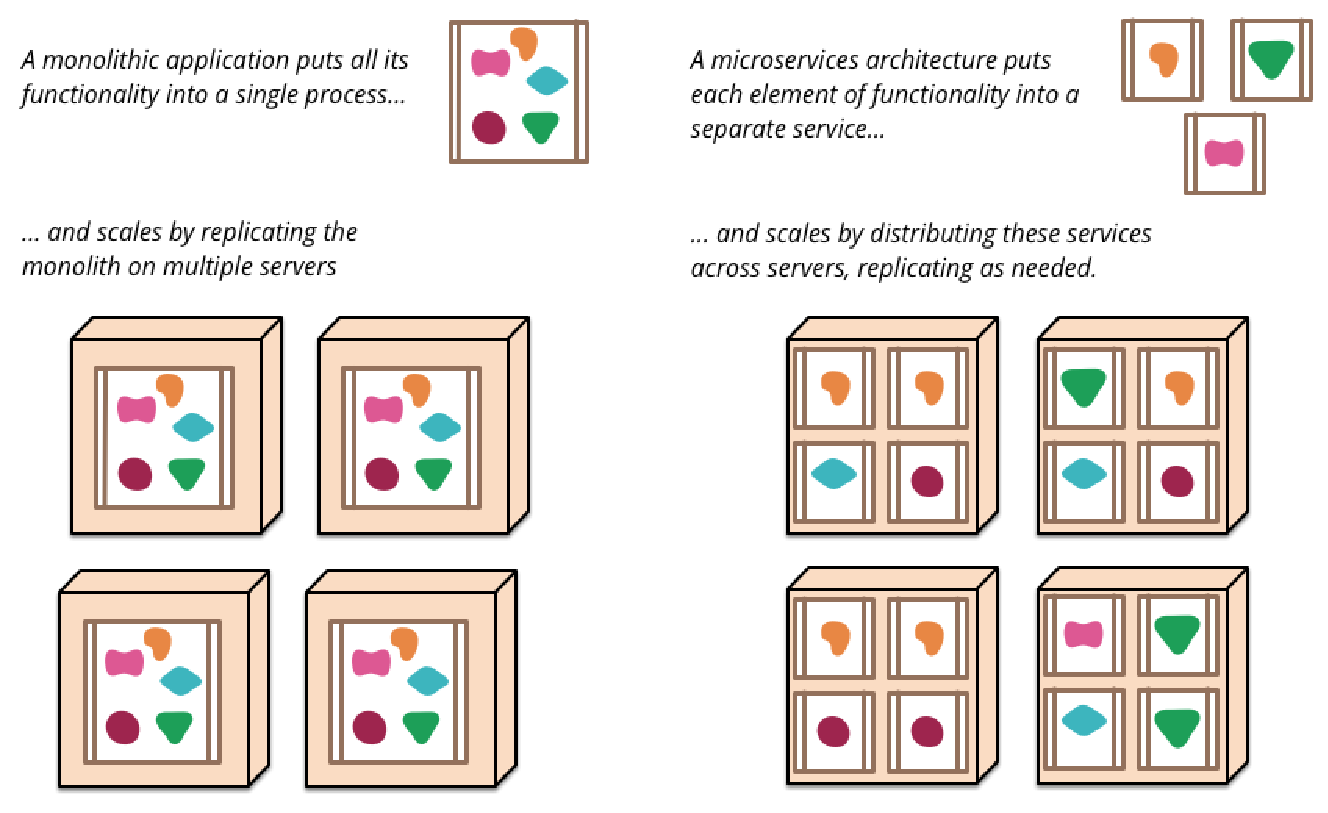
\includegraphics[width=1.00\textwidth]{monolithic_and_microservices.pdf}
    \caption{Monolithic and Microservices architectural styles~\cite{microservices}.}
    \label{fig:monolithic_and_microservices}
\end{figure}

Both styles presented have their own advantages and disadvantages. To briefly present some of them, two examples are provided, one for each architectural style. First example: if one team needs to develop a single process system, e.g., e-Commerce application, that authorizes customer, takes an order, check products inventory, authorize payment and ships ordered products. The best alternative is to use Monolithic architecture, because they can develop every feature in a single software package due to the application simplicity, however, if the client starts to demand hard changes and additional features in the solution, the code base may tend to increase into ``out of control'', leading to more challenging and time consuming changes. Second example, if one team needs to develop a complex and huge service that needs to scale, e.g., Video streaming service, the best alternative is to use Microservices architecture, because they can tackle the problem of complexity by decomposing the application into a set of manageable small services which are much faster to develop and test by individual organized teams, and thus, it will be easier to maintain the code base due to decoupling, however, it will be harder to monitor and manage the entire platform due to additional complexity associated with distributed systems.

Taking into consideration this increasing difficulty in monitoring and managing large Microservice based platforms, one must be aware and observe system behaviour to be able to control it. Therefore, in the next Subsection~\ref{subsec:observability_and_controlling_performance}, the core concept of~\nameref{subsec:observability_and_controlling_performance} is explained.

\subsection{Observability and Controlling Performance}
\label{subsec:observability_and_controlling_performance}

This Subsection aims to provide an introduction to some theory concepts about Observability and Performance Controlling, regarding distributed software systems.

Observability is a meaningfully extension of the word observing. Observing is ``to be or become aware of, especially through careful and directed attention; to notice'~'\cite{observing_definition}. The term Observability comes from the world of engineering and control theory. Observability is not a new term in the industry, however it has gain more focus in the last years due to \gls{devops} raising. It means by definition ``to measure of how well internal states of a system can be inferred from knowledge of its external outputs''~\cite{observability}. Therefore, if our good old software systems and applications do not adequately externalize their state, then even the best monitoring can fall short.

Controlling in control systems is ``to manage the behaviour of a certain system''~\cite{control_systems}. Controlling and Observability are dual aspects of the same problem~\cite{observability}, as we need to have information to infer state and be able take action. E.g., When observing an exponential increase in the \gls{cpu} load, the system scales horizontally invoking more machines and spreading the work between them to easy handle the work. This is a clear and simple example that conjugates the terms presented, we have: values that are observed ``Observability'' and action that leads to system control ``Controlling Performance''.

When we want to understand the working and behaviour of a system, we need to watch it very closely and pay special attention to all details and information it provides. Microservice based systems produce multiple types of information if instrumented. These type of information are the ones mentioned in Chapter~\ref{chap:introduction}: Monitoring, Tracing and Logging. In this thesis, the goal is to use tracing data thus, this type of produced information is the one to focus.

In the next Subsection~\ref{subsec:distributed_tracing}~-~\nameref{subsec:distributed_tracing}, the type of data mentioned before is presented and explained in detail.

\subsection{Distributed Tracing}
\label{subsec:distributed_tracing}

%\todo{How to introduce Google Dapper~\cite{Sigelman2010}}

Distributed tracing~\cite{Sambasivan2016a} is a method that comes from traditional tracing, but in this case acts in a distributed system at the work-flow level. It is used to profile and monitor applications, especially those built using microservice architectures and, in the end, it can be used to help DevOps teams pinpoint where failures occur and what causes system problems.

From this concept, standards emerged, like the best-known OpenTracing~\cite{open_tracing_data_model_specification}. The OpenTracing standard, follows the model proposed by Fonseca~\textit{et al.}~\cite{fonseca2007x}, which defines traces as a tree of spans, which represent scopes or units of work (i.e., thread, function, service) and follows their executing through the system.

OpenTracing uses dynamic, fixed-width metadata to propagate causality between spans, meaning that each span has a \emph{TraceID} common to all spans of that trace, as well as a \emph{SpanID} and \emph{ParentID} that are used to represent parent/child relationships between them~\cite{sambasivan2014so}.

The standard defines the format for spans and the semantic~\cite{open_tracing_semantic_specification, open_tracing_semantic_conventions} conventions for their content / annotations.

%Usually, the span has an operation name, the start time of the operation, its duration and some annotations regarding the operation itself. An example of a span can be an HTTP call or a Remote Procedure Call (RPC). 

Figure~\ref{fig:sample_trace_over_time} provides a clear insight about how spans are related to time and with each other.

\begin{figure}[H]
    \centerline{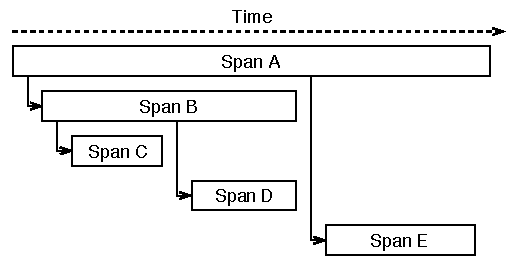
\includegraphics[width=1.0\linewidth]{images/trace.pdf}}
    \caption{Sample trace over time.}
    \label{fig:sample_trace_over_time}
\end{figure}

In Figure~\ref{fig:sample_trace_over_time} there are a group of five spans spread through time that represents a trace. A trace is a group of spans that share the same \emph{TraceID}.  A trace is a representation of a data/execution path in the system. A span represents the logical unit of work in the system. A trace can also be a span, if there is only one span presented in the trace. One span can cause another.

Causality relationship between spans can be observed in Figure~\ref{fig:sample_trace_over_time}, where ``Span A'' causes ``Span B'' and ``Span E'', moreover, ``Span B'' causes ``Span C'' and ``Span D''. From this we say that ``Span A'' is parent of ``Span B'' and ``Span E''. Likewise, ``Span B'' and ``Span E'' are children of ``Span A''. In this case, ``Span A'' does not have a parent, it is an ``orphan span'' and therefore, is the root span and the origin of this whole trace. Spans carry with them metadata like e.g., \emph{SpanID} and \emph{ParentID}, that allows to infer this relationships.

Disposition of spans over time is another clear fact that can be observed from the representation in Figure~\ref{fig:sample_trace_over_time}. Spans have a begin and an end in time. This causes them to have a duration. Spans are spread through time, however they usually stay inside parent boundaries, this means that the duration of a parent span always covers durations of their children. Considering a parent and a child spans, if they are related, the parent span always start before child span, also, the parent span always end after child span. Note that nothing prevents multiple spans to start in the same exact moment. Span also carry with them metadata like e.g., \emph{Timestamp} and \emph{Duration}, that allows to infer their position in time and when they end.

An example of a span can be an \gls{http} call or a \gls{rpc} call. We may think of the following cases to define each operation inherent to each box presented in Figure~\ref{fig:sample_trace_over_time}: A - ``Get user info'', B - ``Fetch user data from database'', C - ``Connect to MySQL server'', D - ``Can't connect to MySQL server'' and E - ``Send error result to client''.

In the data model specification, the creators of OpenTracing say that: ``with a couple of spans, we might be able to generate a span tree and model a directed graph of a portion of the system''~\cite{open_tracing_data_model_specification}. This is due to the causal relationships they represent. Figure~\ref{fig:span_tree_example} provides an example of a span tree.

\begin{figure}[H]
    \centering
    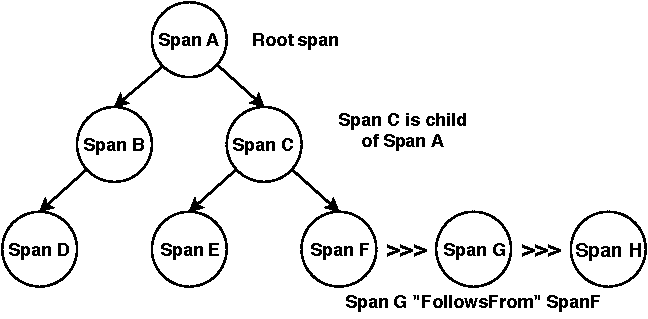
\includegraphics[width=1.0\linewidth]{span_tree_example.pdf}
    \caption{Span Tree example.}
    \label{fig:span_tree_example}
\end{figure}

Figure~\ref{fig:span_tree_example} contains a span tree representation with a trace containing eight spans. As said before,every span must be a child of some other span, unless it is the root span, this is very clear in a span tree visualization with the usage of the root node. With this causal relationship, a path through the system can be retrieved. For example, if for example every span processes in a different endpoint represented by letters presented in the span tree, one may generate the request path: A ---$>$ B ---$>$ D. This means that our hypothetical request passed through machine A, B and D, or if it were services, the request passed from service A, to B and finally to D. From this, we can generate the dependency graph of the system (explained in the Subsection~\ref{subsec:graphs}~-~\nameref{subsec:graphs}).

This type of data is extracted as trace files or streamed over transfer protocols like e.g., \gls{http}, from technologies like Kubernetes~\cite{what_is_kubernetes}, OpenStack~\cite{what_is_opensatck}, and other cloud or distributed management system technologies that implements some kind of system or code instrumentation using, for example, OpenTracing~\cite{what_is_opentracing} or OpenCensus~\cite{what_is_opencensus}. Tracing contains some vital system details as they are the result of system instrumentation and therefore, this data can be used as a resource to provide observability over the distributed system.

As said before, from the causality relationship between spans we can generate a dependency graph of the system. The next Subsection~\ref{subsec:graphs}~-~\nameref{subsec:graphs} aims to provide a clear understand of this concept and how they relate with distributed tracing.

\subsection{Graphs}
\label{subsec:graphs}

From distributed tracing we can be able to extract the system dependency graph from a representative set of traces. To introduce the concept of Graph, ``A Graph is a set of vertices and a collection of directed edges that each connects an ordered pair of vertices''~\cite{graph_standard_definition}.

Taking the very common sense of the term and to provide notation, a graph, $G$, is an ordered pair $G = (V, E)$, where $V$ are the vertices/nodes and $E$ are the edges.

Graphs are defined by:

\begin{itemize}
    \item Node: Are the entities in the graph. They can hold any number of attributes (key-value pairs) called properties. Nodes can be tagged with labels, representing their different roles in a domain. Node labels may also serve to attach metadata (such as index or constraint information) to certain nodes;
    \item Edge (or Relationships): provide directed, named, semantically-relevant connections between two node entities;
    \item Property: can be any kind of metadata attached to a certain Node or a certain Edge.
\end{itemize}

Also, there are multiple types of graphs, they can be:

\begin{enumerate}
    \item Undirected-Graph: the set of edges without orientation between a pair of nodes;
    \item Directed-Graph: the set of edges have one and only one direction between a pair of nodes;
    \item Multi-Directed-Graph: multiple edges have more than one connection between a pair of nodes that represents the same relationship.
\end{enumerate}

Figure~\ref{fig:graphs_types} gives us a simple visual representation of what a graph really is for a more clear understanding.

\begin{figure}[H]
    \centering
    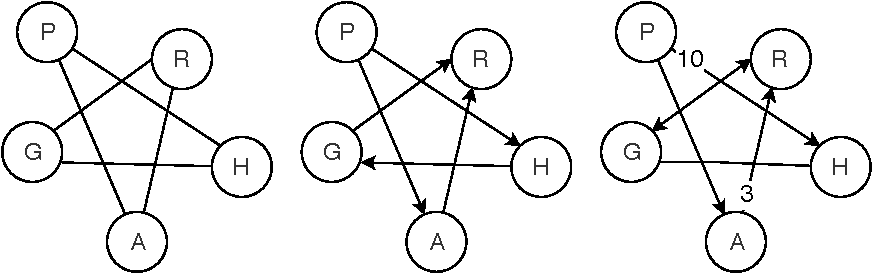
\includegraphics[width=1.00\textwidth]{images/graph_representations.pdf}
    \caption{Graphs types.}
    \label{fig:graphs_types}
\end{figure}

In Figure~\ref{fig:graphs_types} three identical graphs are presented and each one is composed by five nodes, however, they are not equal because each one has it own type. They belong respectively to each type enumerated above. From left to right, the first graph is a Undirected-Graph, the second one is a Directed-Graph and the last one is a Multi-Directed-Graph.

The last graph has some numbers in some edges. Every graph can have this annotations. These can provide some information about the connection between the pair of nodes. For example, in distributed systems context, if this graph represents our system dependency graph, and nodes $H$ and $P$ hypothetical services, the edge between them could represent calls between these two service and the notation number the number of calls with respect to the edge direction. Therefore, in this case, we would have 10 requests from incoming from $P$ to $H$.

Figure~\ref{fig:service_dependency_graph} provides a clear insight about service dependency graphs.

\begin{figure}[H]
    \centering
    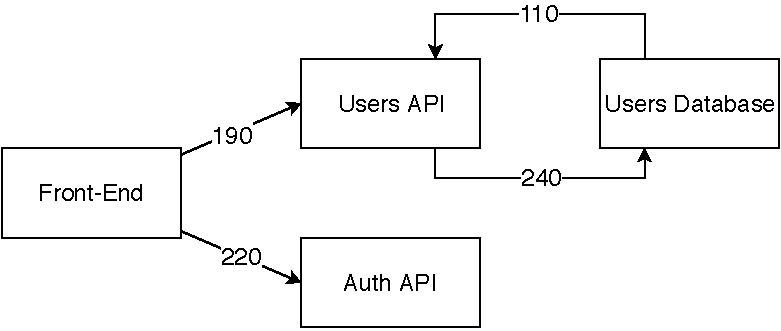
\includegraphics[width=1.00\textwidth]{images/graph_service_representation.pdf}
    \caption{Service dependency graph.}
    \label{fig:service_dependency_graph}
\end{figure}

In Figure~\ref{fig:service_dependency_graph}, a representation of a service dependency graph is provided. Service dependency graphs are graphs of type Multi-Directed-Graph, because they have multiple edges with more than one direction between a pair of services(Nodes). In this representation, there are multiple services involved, each inside a box. The edges between boxes (Nodes), indicate the number of calls that each pair of services invoked, e.g., ``Users API'' called ``Ùsers Database'' 240 times. These dependency graphs gives the state of the system in a given time interval. This can be useful to study the changes in the morphology of the system, e.g., a service disappeared and a set of new ones appeared. Other interesting study could be the variation in the amount of call between services.

Graphs are a way to model and extract information from tracing data. Another interesting approach could be to extract metrics in time from tracing because traces and spans are spread in time, and they have information about the state of the system at a given instant. The next Subsection~\ref{subsec:time_series}~-~\nameref{subsec:time_series} provides an introduction to a data representation model.

\subsection{Time Series}
\label{subsec:time_series}

Time-Series are a way of representing data as a time-indexed series of values. This kind of data is often arise when monitoring systems, industrial processes, tracking corporate business metrics or sensor measurements. Figure~\ref{fig:time_series_example} provides a visual example of this way of data representation.

\begin{figure}[H]
    \centering
    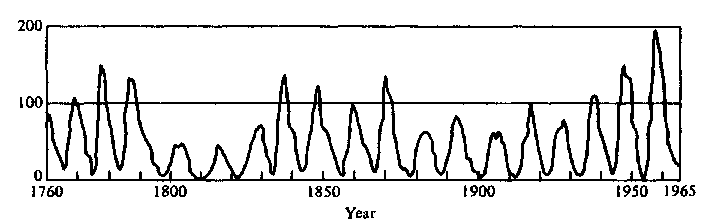
\includegraphics[width=1.00\textwidth]{images/time_series_example.pdf}
    \caption{Time series: Annual mean sunspot numbers for 1760-1965~\cite{Brillinger2006}.}
    \label{fig:time_series_example}
\end{figure}

In Figure~\ref{fig:time_series_example}, Brillinger \textit{D.}~\cite{Brillinger2006} presents a visual representation of a time-series as a collection of values in time. These values are measurements of sunspot means gathered from 1960-1965. In this case, measurements come from natural origin, however, one can perform observations of e.g., \gls{cpu} load, system uptime / downtime and network latency.

As these processes are not random, autocorrelation can be exploited to extract insight from the data, such as predict patterns or detect anomalies. Therefore, time-series data can be analysed to detect anomalies present in the system. One way to do this is to look for outliers~\cite{Liu2004} in the multidimensional feature set. Anomaly detection in time series data is a data mining process used to determine types of anomalies found in a data set and to determine details about their occurrences. Anomaly detection methods are particularly interesting for our data set since it would be impossible to manually tag the set of interesting anomalous points. Figure~\ref{fig:time_series_anomaly_detection_example} provides a simple visual representation of anomaly detection in time series data.

\begin{figure}[H]
    \centering
    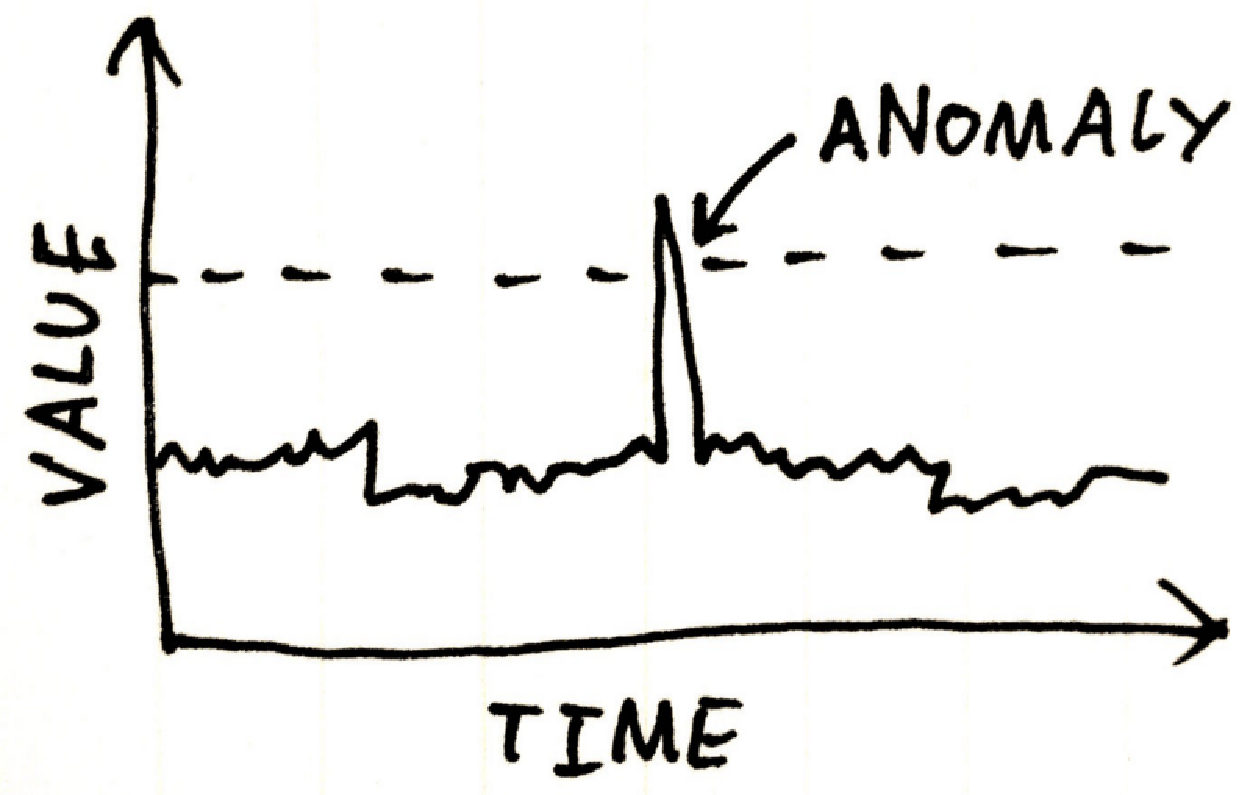
\includegraphics[width=0.50\textwidth]{images/time_series_anomaly_detection_example.pdf}
    \caption{Anomaly detection in Time Series~\cite{NikolajBomannMertz}.}
    \label{fig:time_series_anomaly_detection_example}
\end{figure}

In Figure~\ref{fig:time_series_anomaly_detection_example}, there is a clear spike in values from this time series measurements. This can be declared an outlier because it is a strange value considering the range of remaining measurements and therefore, it is considered an anomaly. In this example, anomaly detection is easy to perform by a Human, however, in mostly cases nowadays, due to great variation of values and plethora of information that can be gathered, perform this detection manually is impracticable, thus automatic anomaly detection using Machine Learning techniques are used nowadays.

Anomaly detection in time series data is a data mining process used to determine types of anomalies found in a data set and to determine details about their occurrences. This auto anomaly detection method has lots of usage due to the impossible work of tag manually the interesting set of anomalous points. Auto anomaly detection has a wide range of applications such as fraud detection, system health monitoring, fault detection, event detection systems in sensor networks, and so on.

After explaining the core concepts, foundations for the work presented in this thesis, to the reader, technologies capable of handling this types of information are presented and discussed in next Section~\ref{sec:technologies}~-~\nameref{sec:technologies}.

\section{Technologies}
\label{sec:technologies}

In this section are presented technologies and tools capable of handling the types of information discussed in the previous Section~\ref{sec:concepts}~-~\nameref{sec:concepts}.

The main tools covered are:~\ref{subsec:distributed_tracing_tools}~-~\nameref{subsec:distributed_tracing_tools}, for distributed tracing data handling, \ref{subsec:graph_manipulation_and_processing_tools}~-~\nameref{subsec:graph_manipulation_and_processing_tools} and~\ref{subsec:graph_database_tools}~-~\nameref{subsec:graph_database_tools}, for graph processing and storage, and~\ref{subsec:time_series_database_tools}~-~\nameref{subsec:time_series_database_tools}, for time series value storage.

\subsection{Distributed Tracing Tools}
\label{subsec:distributed_tracing_tools}

This Subsection presents the most used and known distributed tracing tools. These tools are mainly oriented for tracing distributed systems like microservices-based applications. What they do is to fetch or receive trace data from this kind of complex systems, treat the information, and then present it to the user using charts and diagrams in order to explore the data in a more human-readable way. One of the best features presented in this tools, is the possibility to perform queries on the tracing (e.g., by trace id and by time-frame). Table~\ref{table:distributed_tracing_tools} presents the most well-known open source tracing tools.

\begin{table}[]
    \caption{Distributed tracing tools comparison.}
    \label{table:distributed_tracing_tools}
    \centering
    \begin{tabularx}{\linewidth} {
            >{\hsize=0.70\hsize}X|
            >{\hsize=1.15\hsize}X|
            >{\hsize=1.15\hsize}X|}
        \cline{2-3}

         & Jaeger~\cite{jaeger_github}
         & Zipkin~\cite{zipkin_github} \\ \hline \hline
         \multicolumn{1}{|l|}{\textbf{Brief description}}
         & Released as open source by Uber Technologies and is used for monitoring and troubleshooting microservices-based distributed systems. Was inspired by Zipkin.
         & Helps gather timing data needed to troubleshoot latency problems in microservice architectures and manages both the collection and lookup of this data. Zipkin's design is based on the Google Dapper paper. \\ \hline
         \multicolumn{1}{|l|}{\textbf{Pros}}
         & OpenSource; \newline
        Docker-ready; \newline
        Collector interface is compatible with Zipkin protocol; \newline
        Dynamic sampling rate; \newline
        Browser UI.
         & OpenSource; \newline
        Docker-ready; \newline
        Allows lots of span transport ways (HTTP, Kafka, Scribe, AMQP); \newline
        Browser UI. \\ \hline
        \multicolumn{1}{|l|}{\textbf{Cons}}
         & Only supports two span transport ways (Thrift and HTTP).
         & Fixed sampling rate. \\ \hline
         \multicolumn{1}{|l|}{\textbf{Analysis}}
         & Dependency graph view; \newline
         Trace comparison (End 2018).
         & Dependency graph view. \\ \hline
        \multicolumn{1}{|l|}{\textbf{Used by}}
         & Red Hat; \newline
         Symantec; \newline
         Uber. \newline
         & AirBnb; \newline
         IBM; \newline
         Lightstep. \\ \hline
    \end{tabularx}
\end{table}

In Table~\ref{table:distributed_tracing_tools}, we can see that these two tools are very similar. Both are open source projects, allow docker containerization and provide a browser ui to simplify user interaction. Jaeger was created by Uber and the design was based on Zipkin, however, it does not provide much more features. The best feature that was released for Jaeger in the past year was the capability of perform trace comparison, where the user can select a pair of traces and compare them in terms of structure. This is a good effort in additional features, but it is short in versatility because we can only compare a pair of traces in a ``sea'' of thousands, or even millions.

These tools aim to collect trace information and provide a user interface with some query capabilities for \gls{devops} to use. However they are always focused on span and trace lookup and presentation, and do not provide a more interesting analysis of the system, for example to determine if there is any problem related to some microservice presented in the system. This kind of work falls into the user, \gls{devops}, as they need to perform the tedious work of investigation and analyse the tracing with the objective of find anything wrong with them.

This kind of tools can be a good starting point for the problem that we face, because they already do some work for us like grouping the data generated by the system and provide a good representation for them.

In next Subsection~\ref{subsec:graph_manipulation_and_processing_tools}, graph manipulation and processing tools are presented and discussed.

\subsection{Graph Manipulation and Processing Tools}
\label{subsec:graph_manipulation_and_processing_tools}

Distributed tracing is a type of data produced by Microservice based architectures. This type of data is composed by traces and spans. With a set of related spans, a service dependency graph can be produced. This dependency graph is a Multi-Directed-Graph, as presented in Subsection~\ref{subsec:graphs}. Therefore, with this data at our disposal, there is the need of a graph manipulation and processing tool.

In this Subsection, graph manipulation


\todo{CONTINUE FROM HERE!!!}

Considering that we have data to be processed and manipulated, we have to be sure that we can handle it for analysis. For this purpose, and knowing that the data is a representation and an abstraction of a graph, we needed to study the frameworks available this task. Table~\ref{table:graph_manipulation_and_processing_tools_comparison} presents the main technologies available at the time for graph manipulation and processing.

\begin{table}[H]
    \caption{Graph manipulation and processing tools comparison.}
    \label{table:graph_manipulation_and_processing_tools_comparison}
    \centering
    \begin{tabularx}{\linewidth} {
            >{\hsize=0.1\hsize}X|
            >{\hsize=1.0\hsize}X|
            >{\hsize=1.0\hsize}X|
            >{\hsize=1.0\hsize}X|}
        \cline{2-4}

        & Apache Giraph \cite{apache_giraph}
        & Ligra \cite{ligra_graph_processing_framework}
        & NetworkX \cite{networkx} \\ \hline \hline
         \multicolumn{1}{|l|}{\textbf{Description}}
         & An iterative graph processing system built for high scalability. Currently used at Facebook to analyse the social graph formed by users and their relationships.
         & A library collection for graph creation, analysis and manipulation of networks.
         & A Python package for the creation, manipulation, and study of structure, dynamics, and functions of complex networks. \\ \hline
         \multicolumn{1}{|l|}{\textbf{Licence}~\cite{Morin2012}}
         & Free Apache 2.
         & MIT.
         & BSD - New License. \\ \hline
        \multicolumn{1}{|l|}{\textbf{Supported languages}}
         & Java and Scala.
         & C and C++.
         & Python. \\ \hline
         \multicolumn{1}{|l|}{\textbf{Pros}}
         & Distributed and very scalable; \newline
        Excellent performance -- Process one trillion edges using 200 modest machines in 4 minutes.
         & Handles very large graphs; \newline
        Exploit large memory and multi-core \gls{cpu} -- Vertically scalable.
         & Good support and very easy to install with Python; \newline
        Lots of graph algorithms already implemented and tested. \newline \\ \hline
        \multicolumn{1}{|l|}{\textbf{Cons}}
        & Uses ``Think-Like-a-Vertex'' programming model that often forces into using sub-optimal algorithms, thus is quite limited and sacrifices performance for scaling out; \newline
        Unable to perform many complex graph analysis tasks because it primarily supports Bulk synchronous parallel.
         & Lack of documentation and therefore, very hard to use; \newline
        Does not have many usage in the community.
         & Not scalable (single-machine); \newline
        High learning curve due to the maturity of the project; \newline
        Begins to slow down when processing high amount of data -- 400.000+ nodes. \\ \hline
    \end{tabularx}
\end{table}

With the information presented in the previous table, we can have a notion that this three frameworks don't work and perform in the same level in many ways.

One thing to consider when comparing them is the scalability and performance that each can provide, for instance, in this component the first one, Apache Giraph is the winner since it is implemented with the distributed systems paradigm in mind and can scale to multiple-machines to get the job done in no time, considering high amounts of data. In other way, we have the third framework, called NetworkX, that is different from the previous as it works in a single-machine and doesn't have the ability to scale to multiple-machines. This can be a very problematic feature if we are dealing with very high amounts of data and we have to process it in short amounts of time. The last framework, called Ligra, works in a single-machine environment like the previous one, but it can scale vertically as it has the benefit of use and exploit multi-core \gls{cpu}'s.

The second, and also most important thing to consider, is the support and quantity of implemented graph algorithms in the framework, and in this field the tables turned, and the NetworkX has a lot of advantage as it have lots of implemented graph algorithms defined and studied in graph and networking theory. The remaining frameworks don't have very support either because they don't have it documented or because the implementation and architecture that where considered don't allow to implement it.

For a more clear insight of the position of the presented technologies in the previous table, we have the figure \ref{fig:graph_manipulation_and_performance_tools_diagram_comparison}.

\begin{figure}
    \centering
    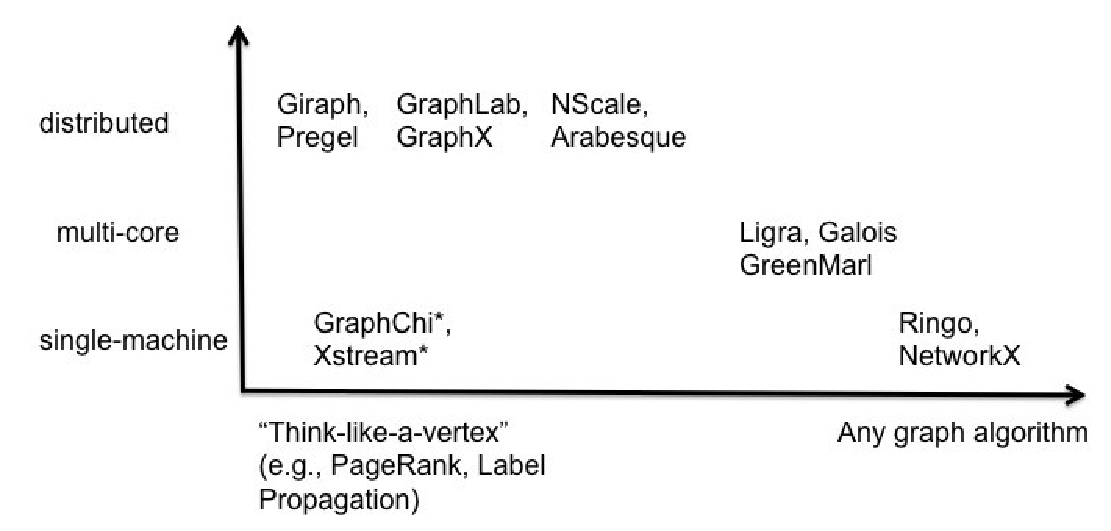
\includegraphics[width=1.0\linewidth]{images/graph_manipulation_tools_diagram_comparison.pdf}
    \caption{Graph manipulation tools comparison, regarding scalability and graph algorithms~\cite{graph_data_management_systems}.}
    \label{fig:graph_manipulation_and_performance_tools_diagram_comparison}
\end{figure}

With the presented figure, our perception of what we might choose when considering this tools is more clear, but we have always some trade offs we cannot avoid. The best approach, and if it's possible, is to consider the usage of an hybrid environment where Giraph and NetworkX coexist one with another, as one fills the gaps of the other, but always taking into consideration that a bottleneck will occur between them \cite{graph_frameworks_performance_evaluation} and that there are almost none implementation where they coexist \cite{graph_frameworks_performance_evaluation} because of their disparity.

\subsection{Graph Database Tools}
\label{subsec:graph_database_tools}

\todo{This data can be modelled as information. After having a Graph instantiated we may be able to store it. For this type of information, there are specific ways of storing it. For example, we can store graphs in a \gls{gdb}. A \gls{gdb} is ``a database that uses graph structures for semantic queries with nodes, edges and properties to represent and store data''\cite{graph_database_definition}.}

Manipulating and process graph data is not enough, we need to store this data somewhere, and to do this we need a \gls{gdb}. The results of the research for the best graph databases tools available are presented in the table \ref{table:graph_databases_comparison}.

\begin{table}[!b]
    \caption{Graph databases comparison.}
    \label{table:graph_databases_comparison}
    \centering
    \large
    \begin{tabularx}{\linewidth} {
        |>{\hsize=0.7\hsize}X|
        >{\hsize=1.1\hsize}X|
        >{\hsize=1.1\hsize}X|
        >{\hsize=1.1\hsize}X| }
        \hline
        \textbf{Name}
         & ArangoDB \cite{arangodb_documentation}
         & Facebook TAO \cite{facebook_tao_article}
         & Neo4J \cite{neo4j_documentation}                                                                                                                                                                                 \\ \hline
        \textbf{Description}
         & It's a NoSQL database developed by ArangoDB Inc. that uses a proper query language to access the database.
         & TAO, “The Associations and Objects”, is a proprietary database, developed by Facebook, that stores all the data related to the users in the social network.
         & It's the most popular open source graph database. Has been developed by Neo4J Inc. and is completely open to the community.                                                                                      \\ \hline
        \textbf{Licence}
         & Free Apache 2
         & Proprietary
         & GPLv3 CE                                                                                                                                                                                                         \\ \hline
        \textbf{Supported languages}
         & C++ \newline
        Go \newline
        Java \newline
        JavaScript \newline
        Python \newline
        Scala
         & \centering -----
         & Java \newline
        JavaScript \newline
        Python \newline
        Scala                                                                                                                                                                                                               \\ \hline
        \textbf{Pros}
         & Multi data-type support (key/value, documents, graphs). Allows the combination of different data access patterns in a single query. Supports cluster deployment.
         & Very fast(~=100ms latency). Accepts millions of calls per second. Distributed.
         & Supports ACID(Atomicity, Consistency, Isolation, Durability)\cite{acid_definition}. High-availability. Has a visual node-link graph explorer. REST \gls{api} interface. Most popular open source graph database. \\ \hline
        \textbf{Cons}
         & Needed to learn a new query language called AQL(Arango Query Language). High learning curve. Has paid version with high price tag.
         & Not accessible to use.
         & Can’t be distributed (It needs to be vertically scaled).                                                                                                                                                         \\ \hline
    \end{tabularx}
\end{table}

As we can notice by the data provided by the presented table, the state of the art about graph databases is not very good. The offers are very limited and all of them lack something when we start to see them in detail. The interest in this databases is increasing as graph technology tend to have many use cases and solve lots of problems nowadays.

Facebook detains the most powerful and robust system for this purpose, but as it is the base of their business because they need to perform large operations in their huge social graph in reduced times, it is a proprietary technology and is only referenced in some articles \cite{facebook_tao_article}.

The remaining two tools, are very supported by the community because of their license and demand, however based on the stars and forks of their repositories, Neo4J is more well received by the community and tends to become more popular. It doesn't implement horizontal scalability by design and this can be a risk when using it in systems with scalabilty in mind, but there are some authors that report they were able to perform implementations and surpass the scalability issue, however with many snags\cite{neo4j_scalable}. ArangoDB supports scalability by default as we can see in the figure \ref{fig:arangodb_vs_neo4j_scalability}\cite{arangodb_vs_ne4j}, but it has a very hard query language with a high learning curve inherent to it, and it is payed to use some special features like SmartGraphs storage\cite{arangodb_smart_graphs} that improves the writing of graph in distributed databases.

\begin{figure}[H]
    \centering
    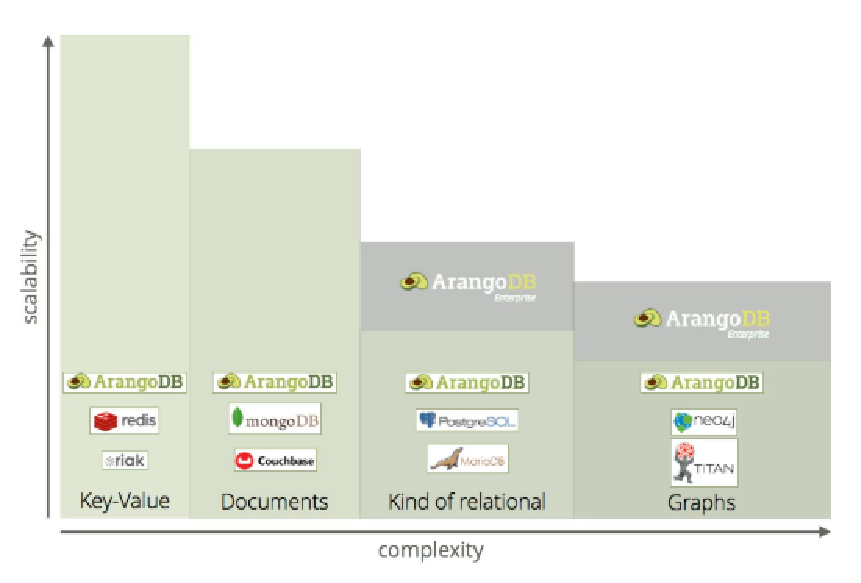
\includegraphics[width=0.80\textwidth]{images/arangodb_vs_neo4j_scalability.pdf}
    \caption{ArangoDB vs. Neo4J scalability over complexity.}
    \label{fig:arangodb_vs_neo4j_scalability}
\end{figure}

\subsection{Time-Series Database Tools}
\label{subsec:time_series_database_tools}

\todo{CHECK THIS!!!}

A \gls{tsdb} is ``is a database optimised for time-stamped or time series data like arrays of numbers indexed by time (a date time or a date time range)''\cite{time_series_database_definition}.

This kind of databases are natively implemented using specialised database algorithms to enhance it's performance and efficiency due to the widely variance of access possible. The way this databases use to work on efficiency is to treat time as a discrete quantity rather than as a continuous mathematical dimension. Usually a \gls{tsdb} allows operations like create, enumerate, update, organise and destroy various time series entries.

The \gls{tsdb} and the \gls{gdb}, presented in this subsection and in the subsection before respectively, are at the time, the most wanted and fastest growing kind of databases due to their use cases in the trending fields of Cloud and Distributed based Systems and in the \textit{Internet of Things (IoT)}. The figure \ref{fig:fastest_growing_databases} presents the growing of this databases in the last two years. As we can see in the figure presented, the \gls{tsdb} and \gls{gdb} are distancing from the remaining databases in terms of popularity starting from the same spot in December of 2016. The predictions are that this databases will not stop increasing popularity, until this kind of systems described before start losing it too.

\begin{figure}
    \centering
    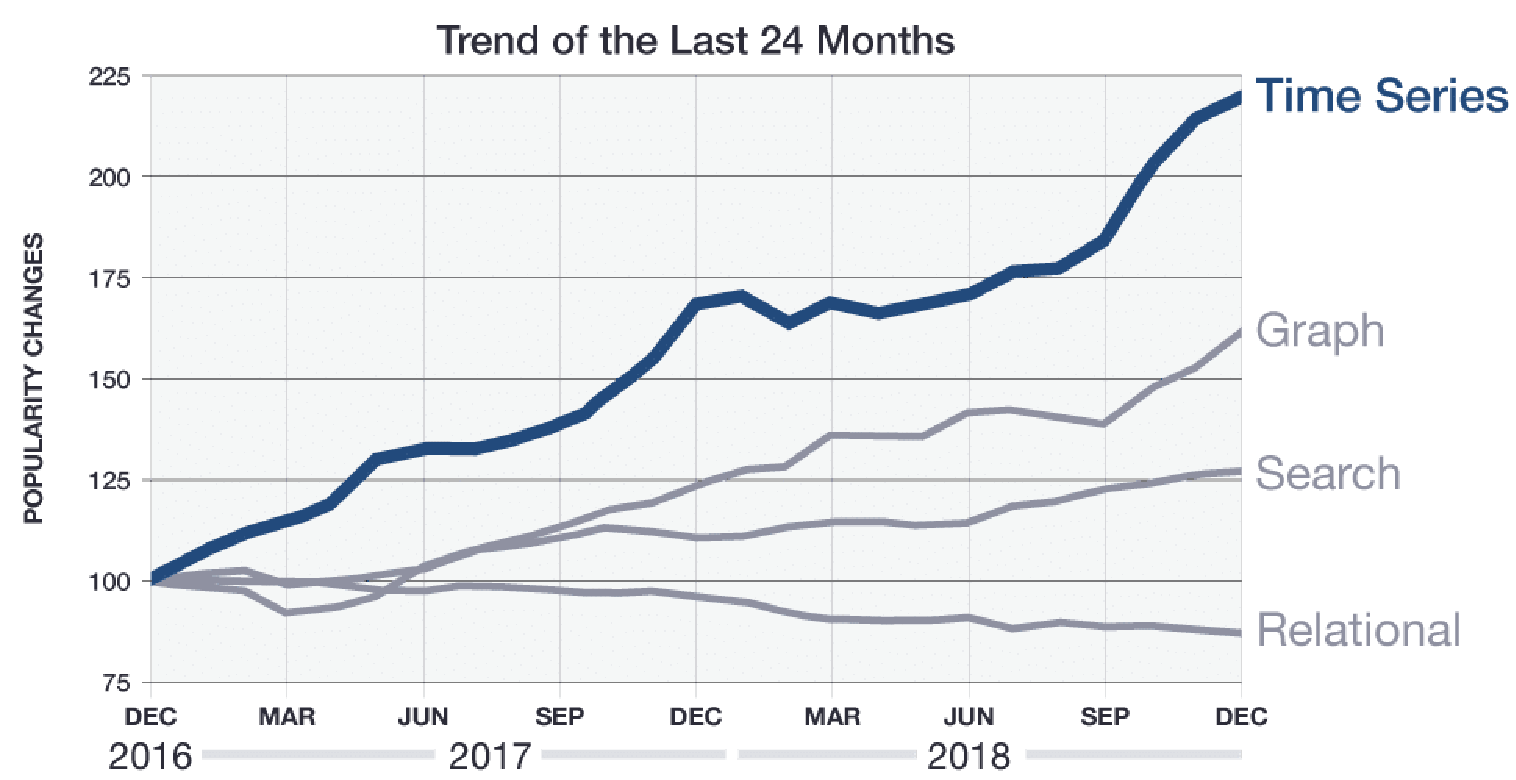
\includegraphics[width=1.0\textwidth]{images/popularity_of_time_series_databases.pdf}
    \caption{Fastest Growing Databases.\cite{time_series_databases_explained}}
    \label{fig:fastest_growing_databases}
\end{figure}

\todo{CHECK THIS!!!}

As we intend to extract useful data from span trees and graphs, we need to store it somewhere. We already know that the spans and trace data are directly related with time based information, explained in the subsection \ref{subsec:traces_and_spans} - \nameref{subsec:traces_and_spans}, so the best way to store the gathered or calculated information from them is in a \gls{tsdb}.

The figure \ref{fig:time_series_databases_ranking} present the ranking of the \gls{tsdb} at the current time\cite{tsdb_ranking}.

\begin{figure}[h!]
    \centering
    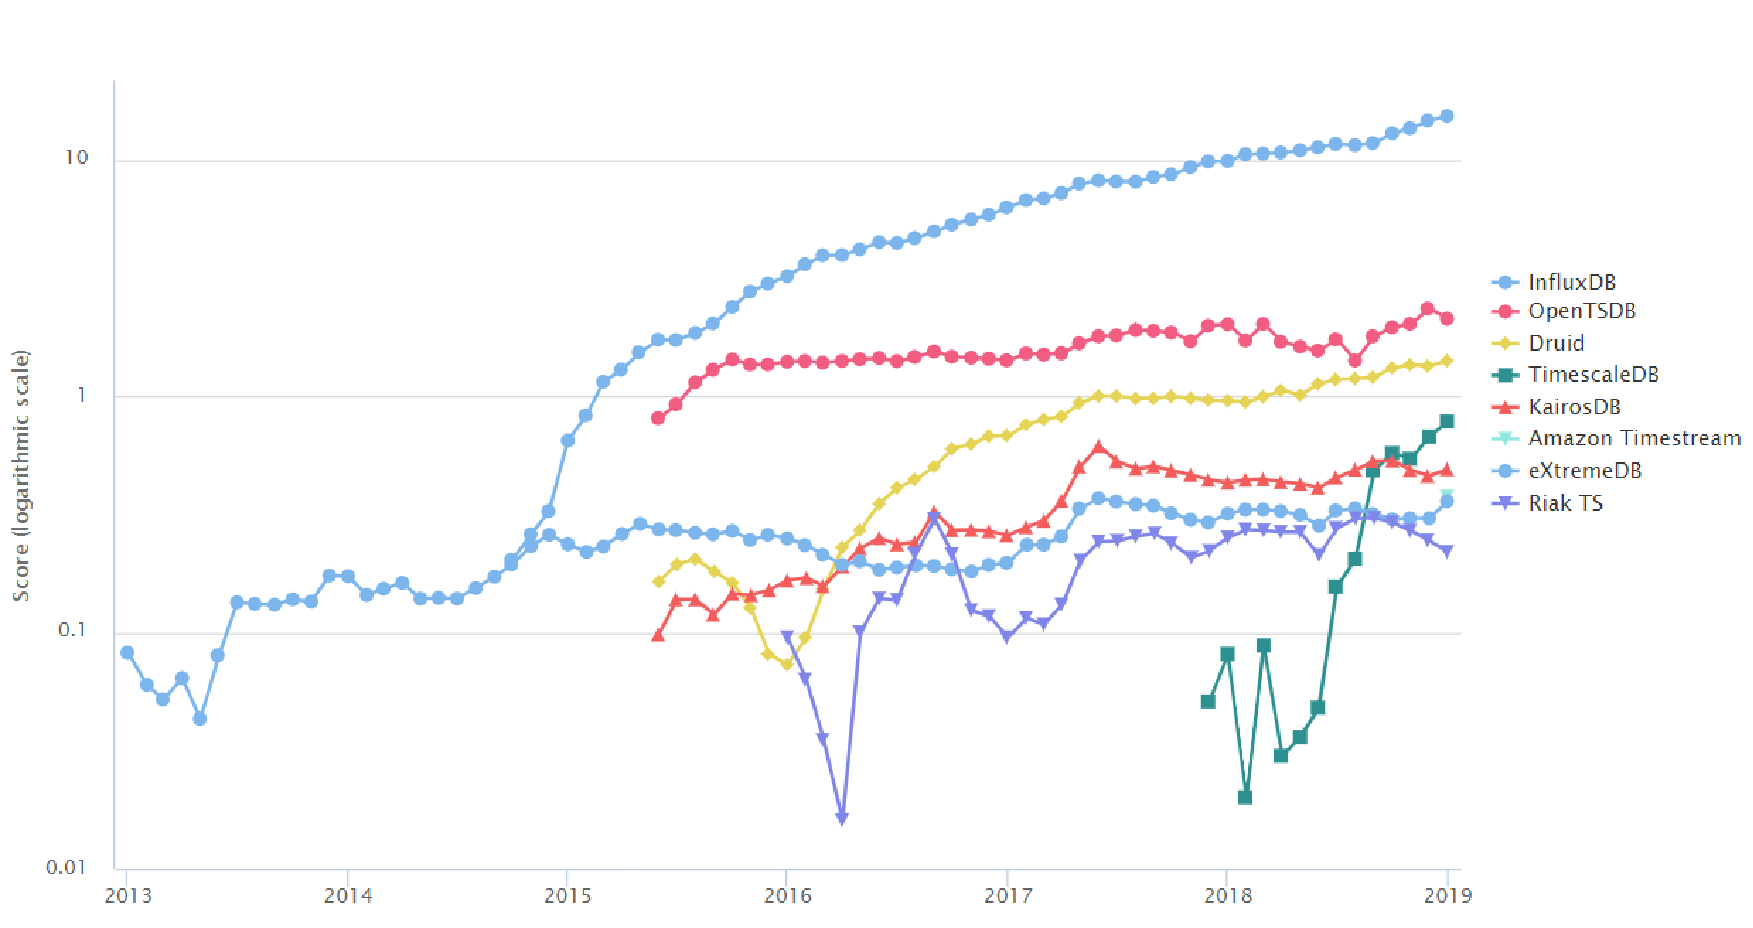
\includegraphics[width=1.00\textwidth]{images/time_series_databases_ranking.pdf}
    \caption{\gls{tsdb}s ranking from 2013 to 2019.}
    \label{fig:time_series_databases_ranking}
\end{figure}

The table \ref{table:time_series_databases_comparison} exposes a comparison between the two top databases presented in the ranking, the \textit{InfluxDb} and \textit{OpenTSDB}, two very well known databases in the world of \gls{tsdb}, in order to understand the advantages and disadvantages of each one.

\begin{table}[H]
    \caption{Time-series databases comparison.}
    \label{table:time_series_databases_comparison}
    \centering
    \large
    \begin{tabularx}{\linewidth} {
        |>{\hsize=0.50\hsize}X|
        >{\hsize=1.25\hsize}X|
        >{\hsize=1.25\hsize}X| }
        \hline
        \textbf{Name}
         & InfluxDB \cite{influxdb}
         & OpenTSDB \cite{opentsdb}                                                                                                                                                                                                                                                                                               \\ \hline
        \textbf{Description}
         & It is an open-source time series database developed by InfluxData written in Go and optimised for fast, high-availability storage and retrieval of time series data in fields such as operations monitoring, application metrics, Internet of Things sensor data, and real-time analytics.
         & It is a distributed, scalable Time Series Database (TSDB) written on top of HBase. OpenTSDB was written to address a common need: store, index and serve metrics collected from computer systems (network gear, operating systems, applications) at a large scale, and make this data easily accessible and graphable. \\ \hline
        \textbf{Licence}
         & MIT
         & GPL                                                                                                                                                                                                                                                                                                                    \\ \hline
        \textbf{Supported languages}
         & Erlang \newline
        Go \newline
        Java \newline
        JavaScript \newline
        Lisp \newline
        Python \newline
        R \newline
        Scala
         & Erlang \newline
        Go \newline
        Java \newline
        Python \newline
        R \newline
        Ruby                                                                                                                                                                                                                                                                                                                      \\ \hline
        \textbf{Pros}
         & Scalable in the enterprise version. \newline
        Outstanding high performance. \newline
        Accepts data via HTTP, TCP, and UDP protocols. \newline
        SQL like query language. \newline
        Allows real-time analytics.
         & It's massively scalable. \newline
        Great for large amounts of time-based events or logs. \newline
        Accepst data via HTTP and TCP access protocols. \newline
        Good platform for future analytical research into particular aggregations on event/log data. \newline
        Doesn't have paid version.                                                                                                                                                                                                                                                                                                \\ \hline
        \textbf{Cons}
         & Enterprise high price tag. \newline
        Clustering support only available in the enterprise version.
         & Expensive to try. \newline
        Not a good choice for general-purpose application data.                                                                                                                                                                                                                                                                   \\ \hline
    \end{tabularx}
\end{table}

Based on the information presented in the referenced table, we can notice that this two databases are very similar on what they offer like the access protocols and scalability capabilities. In the point of licence, both are open source, however the first one, InfluxDB, has an enterprise paid version that is not very well exposed in its documentations and much people don't even notice it, contrarily to OpenTSDB which is completely free. The enterprise version of InfluxDB provides clustering support, high availability and scalability\cite{influxdb_vs_opentsdb}, features that OpenTSDB offer for free, however in terms of performance, InfluxDB outperforms OpenTSDB in almost every benchmark by a far distance as we can see in the figures \ref{fig:influxdb_vs_opentsdb_write_throughput} and \ref{fig:influxdb_vs_opentsdb_storage_requirements}.

\section{Related Work}
\label{sec:related_work}

In this section are presented three section of the existing related work for tracing data analysis. After explaining each one, a brief reflection is made to note some directions of research for this project.

\subsection{Mastering AIOps}
\label{subsec:mastering_aiops}

\todo{// TODO: Explain what is done and how is done.}

\cite{mastering_aiops}

\subsection{Anomaly Detection using Zipkin Tracing Data}
\label{subsec:anomaly_detection_using_zipkin_tracing_data}

\todo{// TODO: Explain what is done and how is done.}

\cite{anomaly_detection_zipkin_tracing_data}

Wei Lee was contacted by email to understand better their research focus, however without success because no answer was given.

\subsection{Analysing distributed trace data}
\label{subsec:analysing_distributed_trace_data}

\todo{// TODO: Explain what is done and how is done.}

\cite{analysisng_distributed_trace_data}

\subsection{Research possible directions}
\label{subsec:research_possible_directions}

\todo{// TODO: Make a brief reflection about the related work.}

After providing the state of the art for this research to the reader, next Chapter~\ref{chap:research_objectives_and_approach}~-~\nameref{chap:research_objectives_and_approach} will cover the objectives of this research, the approach used to tackle the problem and the compiled research questions.

\checkoddpage
\ifthenelse{\boolean{oddpage}}
{ % Odd page
    \newpage
    \blankpage}
{ % Even page
}